\documentclass[tikz, border=10pt]{standalone}
\usetikzlibrary{arrows.meta}

\begin{document}

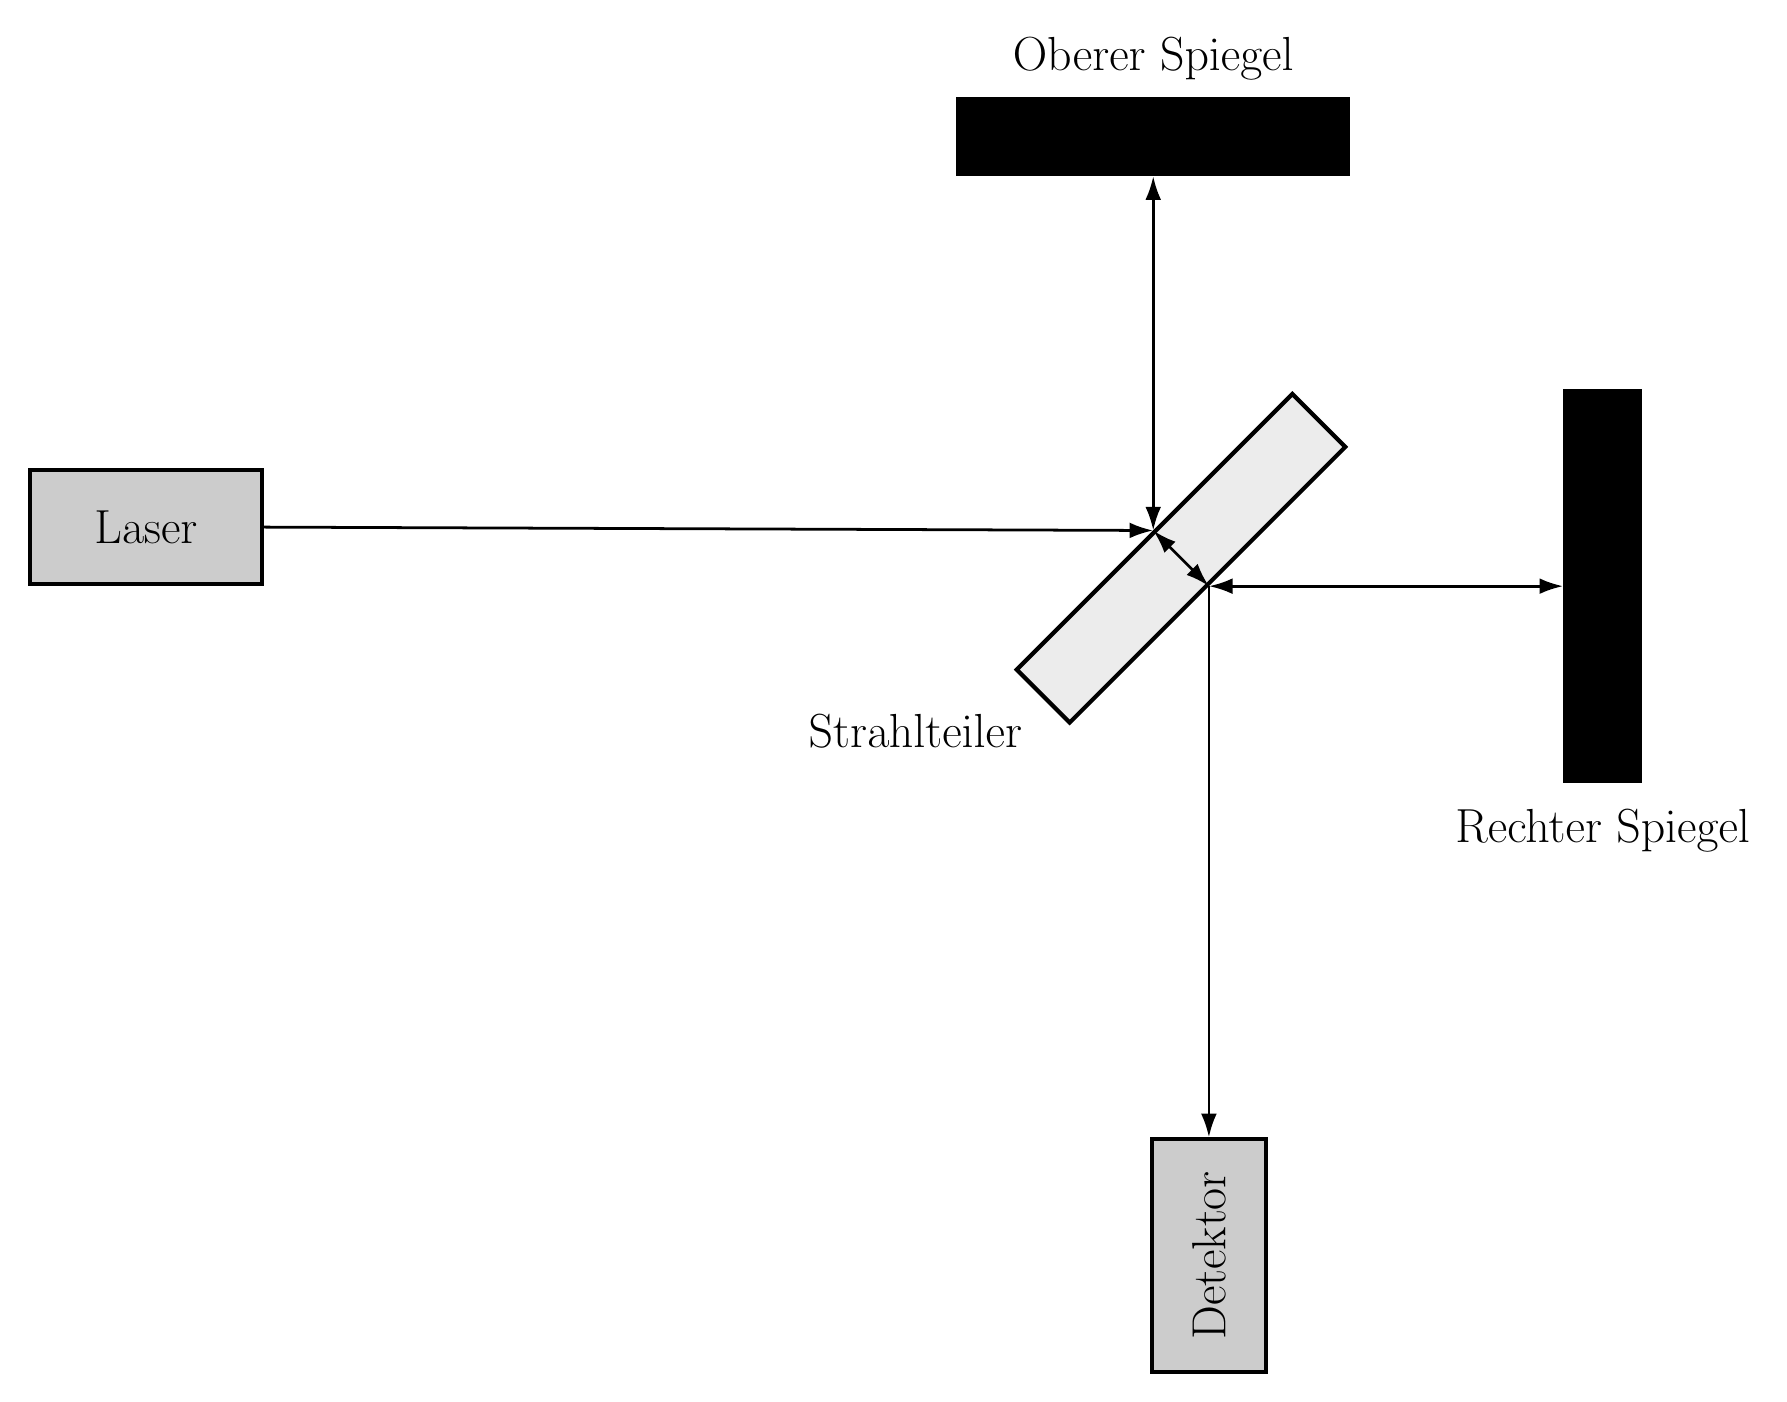
\begin{tikzpicture}

    % --- Grundeinstellungen für Styles ---
    \tikzset{
        % Basis-Stil für alle Komponenten
        component/.style={
            draw, 
            line width=1.5pt, 
            font=\LARGE, 
            align=center
        },
        % Spezifische Komponenten-Stile
        laser/.style={
            component, 
            fill=gray!40, 
            minimum width=2.95cm, 
            minimum height=1.45cm
        },
        detector/.style={
            component, 
            fill=gray!40, 
            minimum width=2.95cm, 
            minimum height=1.45cm
        },
        mirror/.style={
            component, 
            fill=black, 
            minimum width=4.95cm, 
            minimum height=0.95cm
        },
        splitter/.style={
            component, 
            fill=gray!15, 
            minimum width=4.95cm, 
            minimum height=0.95cm, 
            rotate=45
        },
        % Stil für freistehende Beschriftungen
        labeltext/.style={
            font=\LARGE, 
            align=center
        },
        % Stil für Lichtstrahlen
        lightbeam/.style={
            line width=1pt,
            >={Latex[length=3mm, width=2mm]} 
        }
    }

    % --- 1. Optische Komponenten ---

    % Laser
    \node[laser] at (11.5, 12.25) {Laser};

    % Strahlteiler (Mitte)
    \node[splitter] at (24.646, 11.854) {};
    \node[labeltext, anchor=north east, align=right] at (22.75, 10) {Strahlteiler};

    % Rechter Spiegel (gedreht)
    \node[mirror, rotate=90] at (30, 11.5) {};
    % Position angepasst: y von 8.289 auf 7.8 gesetzt (weiter weg)
    \node[labeltext, anchor=south] at (30, 8) {Rechter Spiegel};

    % Oberer Spiegel
    \node[mirror] at (24.293, 17.207) {};
    % Position angepasst: y von 18.418 auf 18.9 gesetzt (weiter weg)
    \node[labeltext, anchor=north] at (24.293, 18.6) {Oberer Spiegel};

    % Detektor
    % Text ist Teil des Nodes und rotiert mit
    \node[detector, rotate=90] at (25, 3) {Detektor};


    % --- 2. Lichtwege (Pfeile) ---
    
    % Strahl zum Detektor
    \draw[lightbeam, <-] (25, 4.5) -- (25, 11.5);

    % Strahl vom Laser zum Strahlteiler
    \draw[lightbeam, ->] (13, 12.25) -- (24.293, 12.207);

    % Strahl zum rechten Spiegel (Hin und Zurück)
    \draw[lightbeam, <->] (24.293, 12.207) -- (25, 11.5);
    \draw[lightbeam, <->] (25, 11.5) -- (29.5, 11.5);

    % Strahl zum oberen Spiegel (Hin und Zurück)
    \draw[lightbeam, <->] (24.293, 12.207) -- (24.293, 16.707);

\end{tikzpicture}

\end{document}